\documentclass[xcolor=pdftex,dvipsnames,table,mathserif]{beamer}
\usepackage{subfigure}
\usepackage{amsbsy}
\usepackage{tikz}
\usetikzlibrary{arrows}
\usepackage{amsmath,graphicx,dsfont,color}
\usepackage{amsfonts}
\usepackage{amssymb}
\usepackage{array}

\bibliographystyle{apalike}

\setbeamertemplate{bibliography item}{\insertbiblabel}
\setbeamertemplate{bibliography entry title}{}
\setbeamertemplate{bibliography entry location}{}
\setbeamertemplate{bibliography entry note}{}

%Definitiona

\newcommand{\x}{\mathbf{x}}
\newcommand{\X}{\mathbf{X}}
\newcommand{\W}{\mathbf{W}} %Weight
\newcommand{\bais}{\mathbf{b}}%Bais
\newcommand{\act}{\texttt{g}}%Activation
\newcommand{\loss}{L}
\newcommand{\pdata}{\hat{p}_{\texttt{data}}}
\newcommand{\nsize}{n}
\newcommand{\param}{\boldsymbol{\theta}}
\newcommand{\featmap}{\boldsymbol{\phi}}
\newcommand{\EV}{\mathbb{E}}







\usepackage{physics}

\graphicspath{{../graphics/}}

%% \usepackage{animate}

\AtBeginSection[]{
  \begin{frame}{Contents}
  \tableofcontents[currentsection, hideothersubsections]
  \end{frame}
}

\AtBeginSubsection[]{
  \begin{frame}{Contents}
  \tableofcontents[currentsection, subsectionstyle=show/shaded/hide]
  \end{frame}
}

\setbeamertemplate{footline}[frame number]{}
\setbeamertemplate{navigation symbols}{}
\setbeamertemplate{section in toc}[square]
\setbeamertemplate{items}[square]

\title{MP10: Deep Learning for Image Analysis\\Course Introduction}
\author{E. Decencière, Thomas Walter, Santiago Velasco-Forero}
\date{MINES ParisTech\\
  PSL Research University
}
\titlegraphic{
\includegraphics[height=1.7cm]{../graphics/logoemp}}

\useinnertheme{rounded}
\usecolortheme{rose}

%%%%%%%%%%%%%%%%%%%%%%%%%%%%%%%%%%%%%%%%%%%%%%%%%%
%%%%%%%%%%%%%%%%%%%%%%%%%%%%%%%%%%%%%%%%%%%%%%%%%%
\begin{document}
\begin{frame}
\titlepage
\end{frame}


%%%%%%%%%%%%%%%%%%%%%%%%%%%%%%%%%%%%%%%%%%%%%%%%%%
\frame{
  \frametitle{About the lecturers}

\begin{columns}
  \begin{column}{.2\textwidth}
\vfill
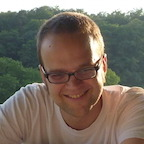
\includegraphics[width=\textwidth]{Thomas_Walter_Heidelberg.jpg}\\
\vspace{2em}
    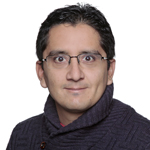
\includegraphics[width=\textwidth]{velascoforero}\\
\vspace{2em}
    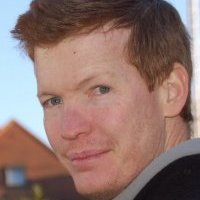
\includegraphics[width=\textwidth]{ed.jpg}

  \end{column}
  \begin{column}{.8\textwidth}

    \begin{block}{Thomas Walter \hfill \scriptsize{\url{http://members.cbio.mines-paristech.fr/\~twalter}}}
      \scriptsize{
    \begin{itemize}
    \item Researcher on bioimage informatics
    \item Main application fields: High Content Screening (HCS), as a method to systematically study biological processes by analyzing cellular phenotypes
    \end{itemize}
    }
  \end{block}

  \begin{block}{Santiago Velasco-Forero  \hfill \scriptsize{\url{http://cmm.mines-paristech.fr/\~velasco}}}
      \scriptsize{
    \begin{itemize}
    \item Researcher on image processing, pattern recognition, multivariate statistics, graph-based data/image analysis
    \item Main application fields: Remote Sensing, cosmetology, astronomy, hyperspectral imaging.
    \end{itemize}
    }
  \end{block}

    \begin{block}{Etienne Decencière \hfill \scriptsize{\url{http://cmm.mines-paristech.fr/\~decenciere}}}
      \scriptsize{
    \begin{itemize}
    \item Researcher on mathematical morphology and image processing
    \item Main application fields: Ophthalmology, dermatology, cosmetology, astronomy
    \end{itemize}
    }
  \end{block}

  \end{column}
\end{columns}



}

%%%%%%%%%%%%%%%%%%%%%%%%%%%%%%%%%%%%
\begin{frame}{Course Team}

  {\scriptsize

\begin{columns}
  \begin{column}{.45\textwidth}

    \begin{block}{Instructors}
      \begin{itemize}
      \item Etienne Decencière
      \item Thomas Walter
      \item Santiago Velasco-Forero
      \end{itemize}
    \end{block}

    \begin{block}{Practical sessions software}
      \begin{itemize}
      \item José-Marcio Martins da Cruz
      \end{itemize}
    \end{block}

  \end{column}

  \begin{column}{.55\textwidth}
    \begin{block}{Teaching assistants}
      \begin{itemize}
        \item Monday: Arthur Imbert
      \item Tuesday: David Duque, Eric Baz\'an
      \item Wednesday: Leonardo Gigli, Eric Baz\'an
      \item Thursday: Bogdan Stanciulescu
      \item Friday: Tristan Lazard
      \end{itemize}
    \end{block}

  \end{column}
\end{columns}


    }

\end{frame}

%%%%%%%%%%%%%%%%%%%%%%%%%%%%%%%%%%%%
\begin{frame}{Program}

\begin{block}{}
  Lectures: 9h-12h30 (\alert{except on Monday: 9h30-12h30})\\
  \hspace{4em}including invited speakers (11h30-12h30)\\
  Practical sessions: 14h-17h30.
\end{block}

% Please add the following required packages to your document preamble:
% \usepackage[table,xcdraw]{xcolor}
% If you use beamer only pass "xcolor=table" option, i.e. \documentclass[xcolor=table]{beamer}
{\tiny
\begin{table}[]
\begin{tabular}{|l|l|l|}
\hline
\rowcolor[HTML]{00009B}
{\color[HTML]{FFFFFF} Day} & {\color[HTML]{FFFFFF} Lecture}                                                                                              & {\color[HTML]{FFFFFF} Invited speaker}                                              \\ \hline
Monday                     & \begin{tabular}[c]{@{}l@{}}Machine learning\\ Artificial neural networks\end{tabular}                                       &                                                                                \\ \hline
Tuesday                    & \begin{tabular}[c]{@{}l@{}}Optimization \\Introduction to Convolutional Neural Networks\end{tabular} & \begin{tabular}[c]{@{}l@{}}Diego Tuccillo\\ Canaries Astrophysics Institute \end{tabular}                  \\ \hline
Wednesday                  & \begin{tabular}[c]{@{}l@{}}Image transformations and semantic segmentation\\ Optimisation\end{tabular}          & \begin{tabular}[c]{@{}l@{}}Maximilian Jaritz\\ Valeo \end{tabular} \\ \hline
Thursday                   & \begin{tabular}[c]{@{}l@{}}Network introspection\\ Applications in robotics\end{tabular}                                    & \begin{tabular}[c]{@{}l@{}}Bogdan Stanciulescu\\ MINES ParisTech\end{tabular}       \\ \hline
Friday                     & Advanced techniques                                                                                                         & \begin{tabular}[c]{@{}l@{}}Olivier Moindrot\\ Owkin\end{tabular}             \\ \hline
\end{tabular}
\end{table}
}

\end{frame}


%%%%%%%%%%%%%%%%%%%%%%%%%%%%%%%%%%%%
\begin{frame}{Grading}

\begin{itemize}
\item Continuous evaluation of practical work
\item Exam (1h30, Friday afternoon)
\end{itemize}

\end{frame}

%%%%%%%%%%%%%%%%%%%%%%%%%%%%%%%%%%%%
\begin{frame}{Main notations}
  \begin{eqnarray*}
    i, j, n, p, q & \hspace{1em} & \text{Integer scalars} \\
    x, y, z & \hspace{1em} & \text{Real scalars} \\
    \x, \y & \hspace{1em} & \text{Real vectors} \\
    \X, \W & \hspace{1em} & \text{Matrices} \\
    f, \act & \hspace{1em} & \text{Functions} \\
    \param & \hspace{1em} & \text{Set of parameters} \\
    \end{eqnarray*}
\end{frame}


%% %%%%%%%%%%%%%%%%%%%%%%%%%%%%%%%%%%%%%%%%%%%%%%%%%%
%% \section*{References}

%% %%%%%%%%%%%%%%%%%%%%%%%%%%%%%%%%%%%%%%%%%%%%%%%%%%

%% \frame[allowframebreaks]{

%% \scriptsize

%% \frametitle{References}

%% %\bibliographystyle{amsalpha}
%% %\bibliographystyle{apalike}

%% \bibliography{edf.bib}

%% \normalsize

%% }

%%%%%%%%%%%%%%%%%%%%%%%%%%%%%%%%%%%%%%%%%%%%%%%%%%
%%%%%%%%%%%%%%%%%%%%%%%%%%%%%%%%%%%%%%%%%%%%%%%%%%
%%%%%%%%%%%%%%%%%%%%%%%%%%%%%%%%%%%%%%%%%%%%%%%%%%

\end{document}
